\documentclass[twocolumn]{article}

\usepackage[left=0.35in,top=0.25in,right=0.35in,bottom=0.25in]{geometry}
\usepackage{amsmath}
\usepackage{minted}
\usepackage{cleveref}
\usepackage{graphicx}
\usepackage{multicol}
\usepackage[no-math]{fontspec}
\setsansfont{Linux Libertine}
\renewcommand{\familydefault}{\sfdefault}
\newcommand{\nl}{\newline}
\newcommand{\hl}{\noindent\rule{\textwidth}{0.5pt}}

\title{Complementary Assignment 1 - INF01009 \\ Intuition on Cross Products}
\author{Guilherme G. Haetinger - 00274702}

\begin{document}

  \maketitle

    \begin{section}{Line Between Points}

      As the specification said, we can have derive a number of things only by
applying cross products to points and lines. One of them, is retrieving the line
function that goes through two points. Defining (\cref{fig:points})

      \begin{align*}
        w &= 1.0 \\
        P1 &= [3, 2, w] \\
        P2 &= [-2, 7, w] \\
        P3 &= [-3, -1, w] \\
        P4 &= [2, 6, w]
      \end{align*}

      \begin{figure}
        \centering
        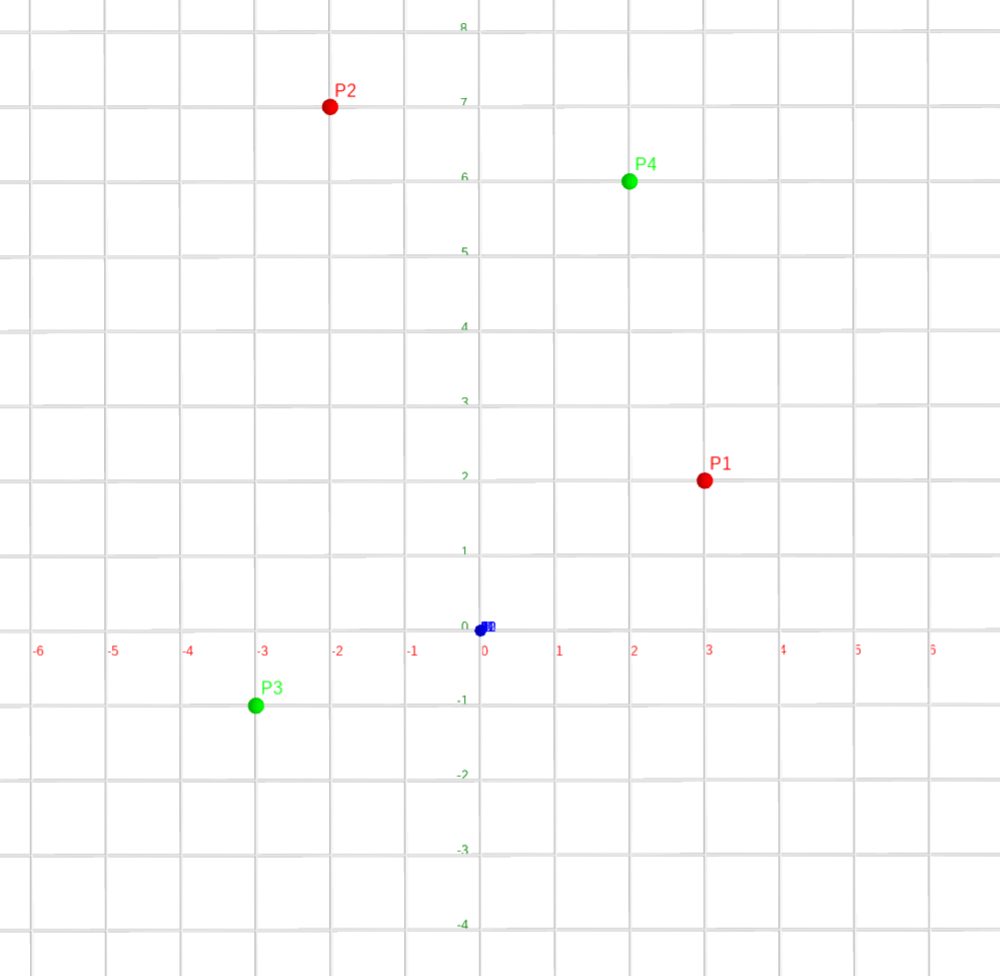
\includegraphics[width=0.85\linewidth]{./res/1.png}
        \caption{Points in the 2D plane}
        \label{fig:points}
      \end{figure}

      Now, we can apply the cross product to find the line equations in a $(a,
b, c) \to ax + by + c = 0$ format:

      \begin{align*}
        L1 = P1 \times P2 = [-5, -5, 25] = [-1, -1, 5] &\to -x -y + 5 = 0 \\
        L2 = P3 \times P4 = [-7, 5, -16] &\to -7x + 5y - 16 = 0
      \end{align*}

      This is rendered as in \cref{fig:lines}.

      \begin{figure}
        \centering
        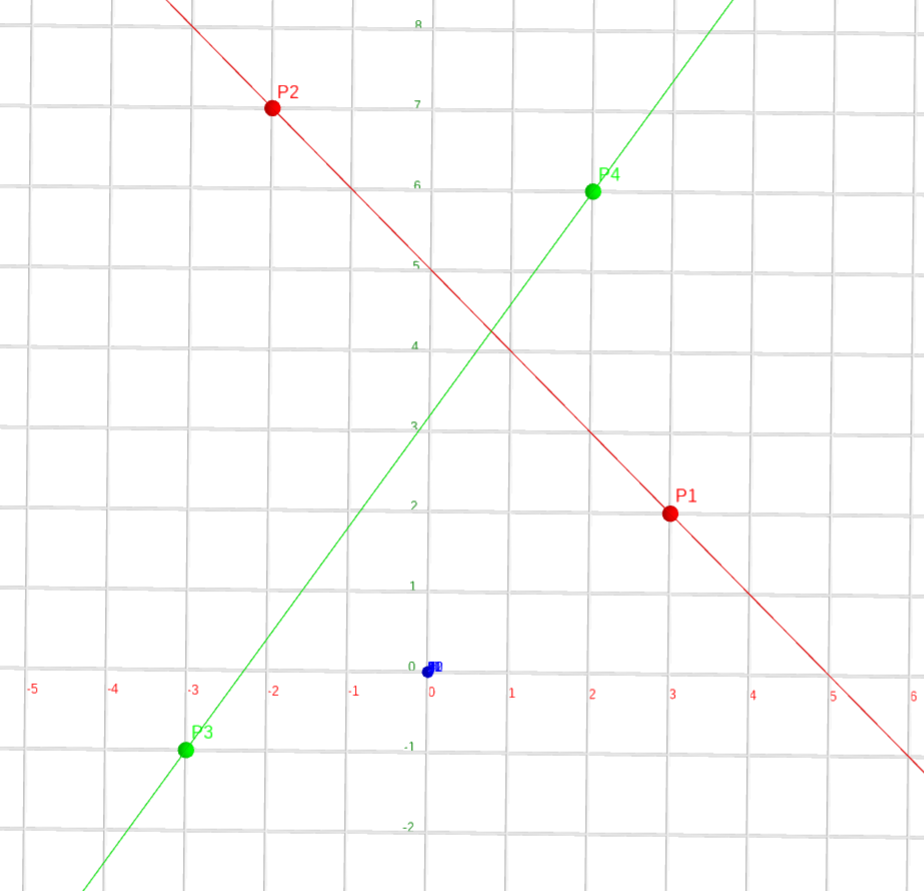
\includegraphics[width=0.85\linewidth]{./res/2.png}
        \caption{Lines in the 2D plane}
        \label{fig:lines}
      \end{figure}

    \end{section}
    \begin{section}{Intersection of Two Lines}

      Now that we have the two lines, we want to find the spot where $-x -y + 2
= -7x +5y - 16$. This can be calculated by working out the equation, or by
calculating the cross product between these two equations' factors. The result
is seen \cref{fig:line-intersection}.

      \begin{figure}
        \centering
        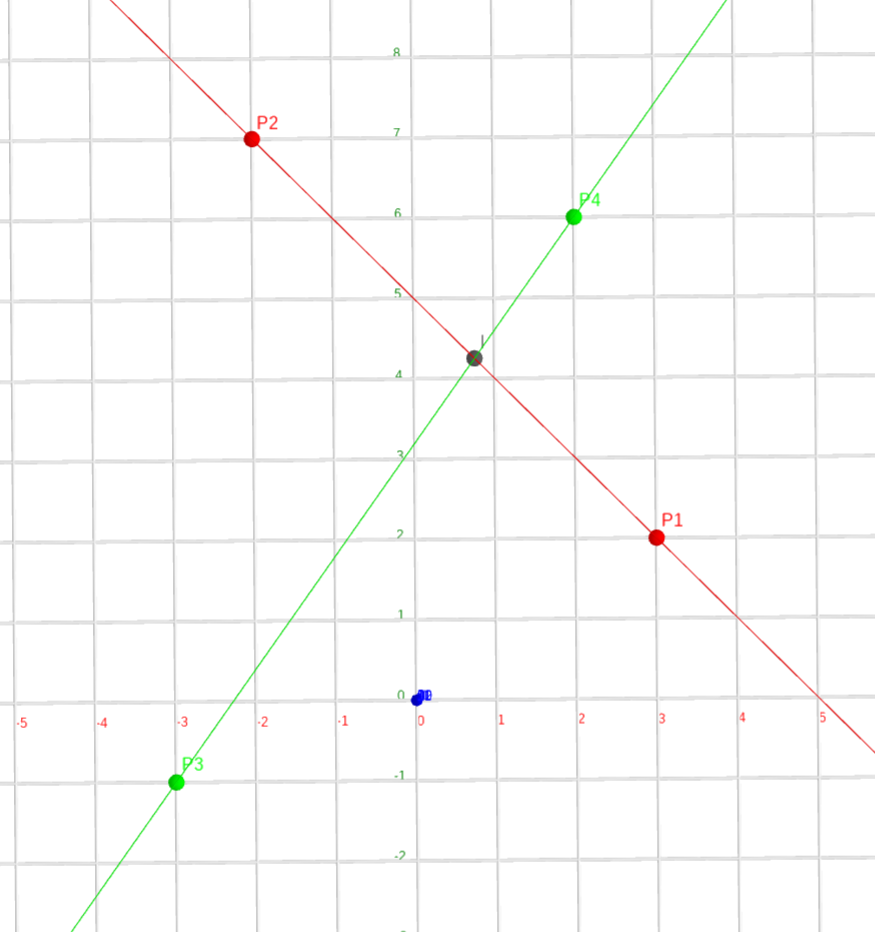
\includegraphics[width=0.85\linewidth]{./res/3.png}
        \caption{Intersection of two lines}
        \label{fig:line-intersection}
      \end{figure}

    \end{section}

    \begin{section}{Defining Planes}
      \label{sec:planes}
      We can define planes for each of these lines. These planes must contain
the two points and the origin ($[0, 0, 0]$). Once they are visible, we can also
render their normals (\cref{fig:planes}).

      \begin{figure}
        \centering
        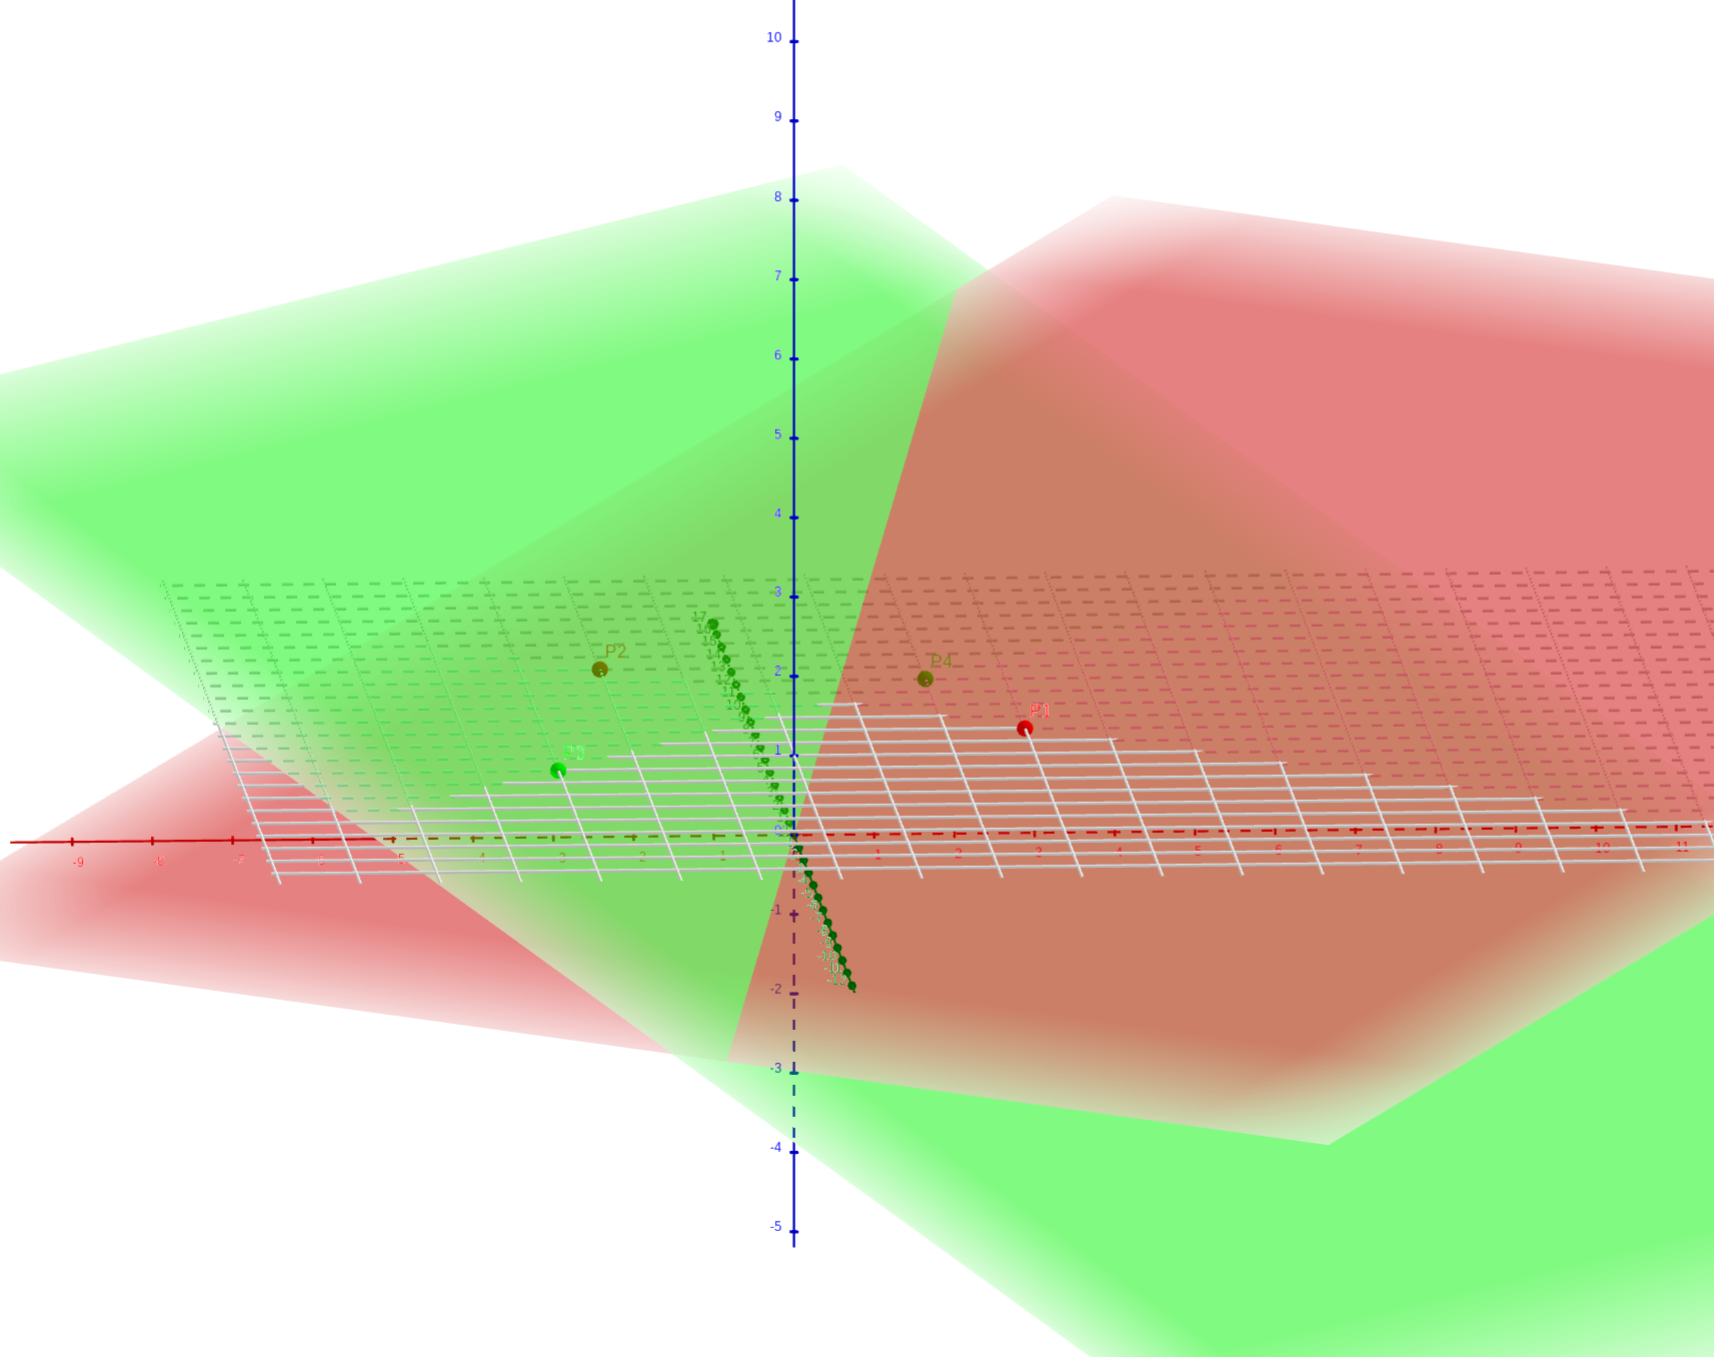
\includegraphics[width=0.49\linewidth]{./res/4.png}
        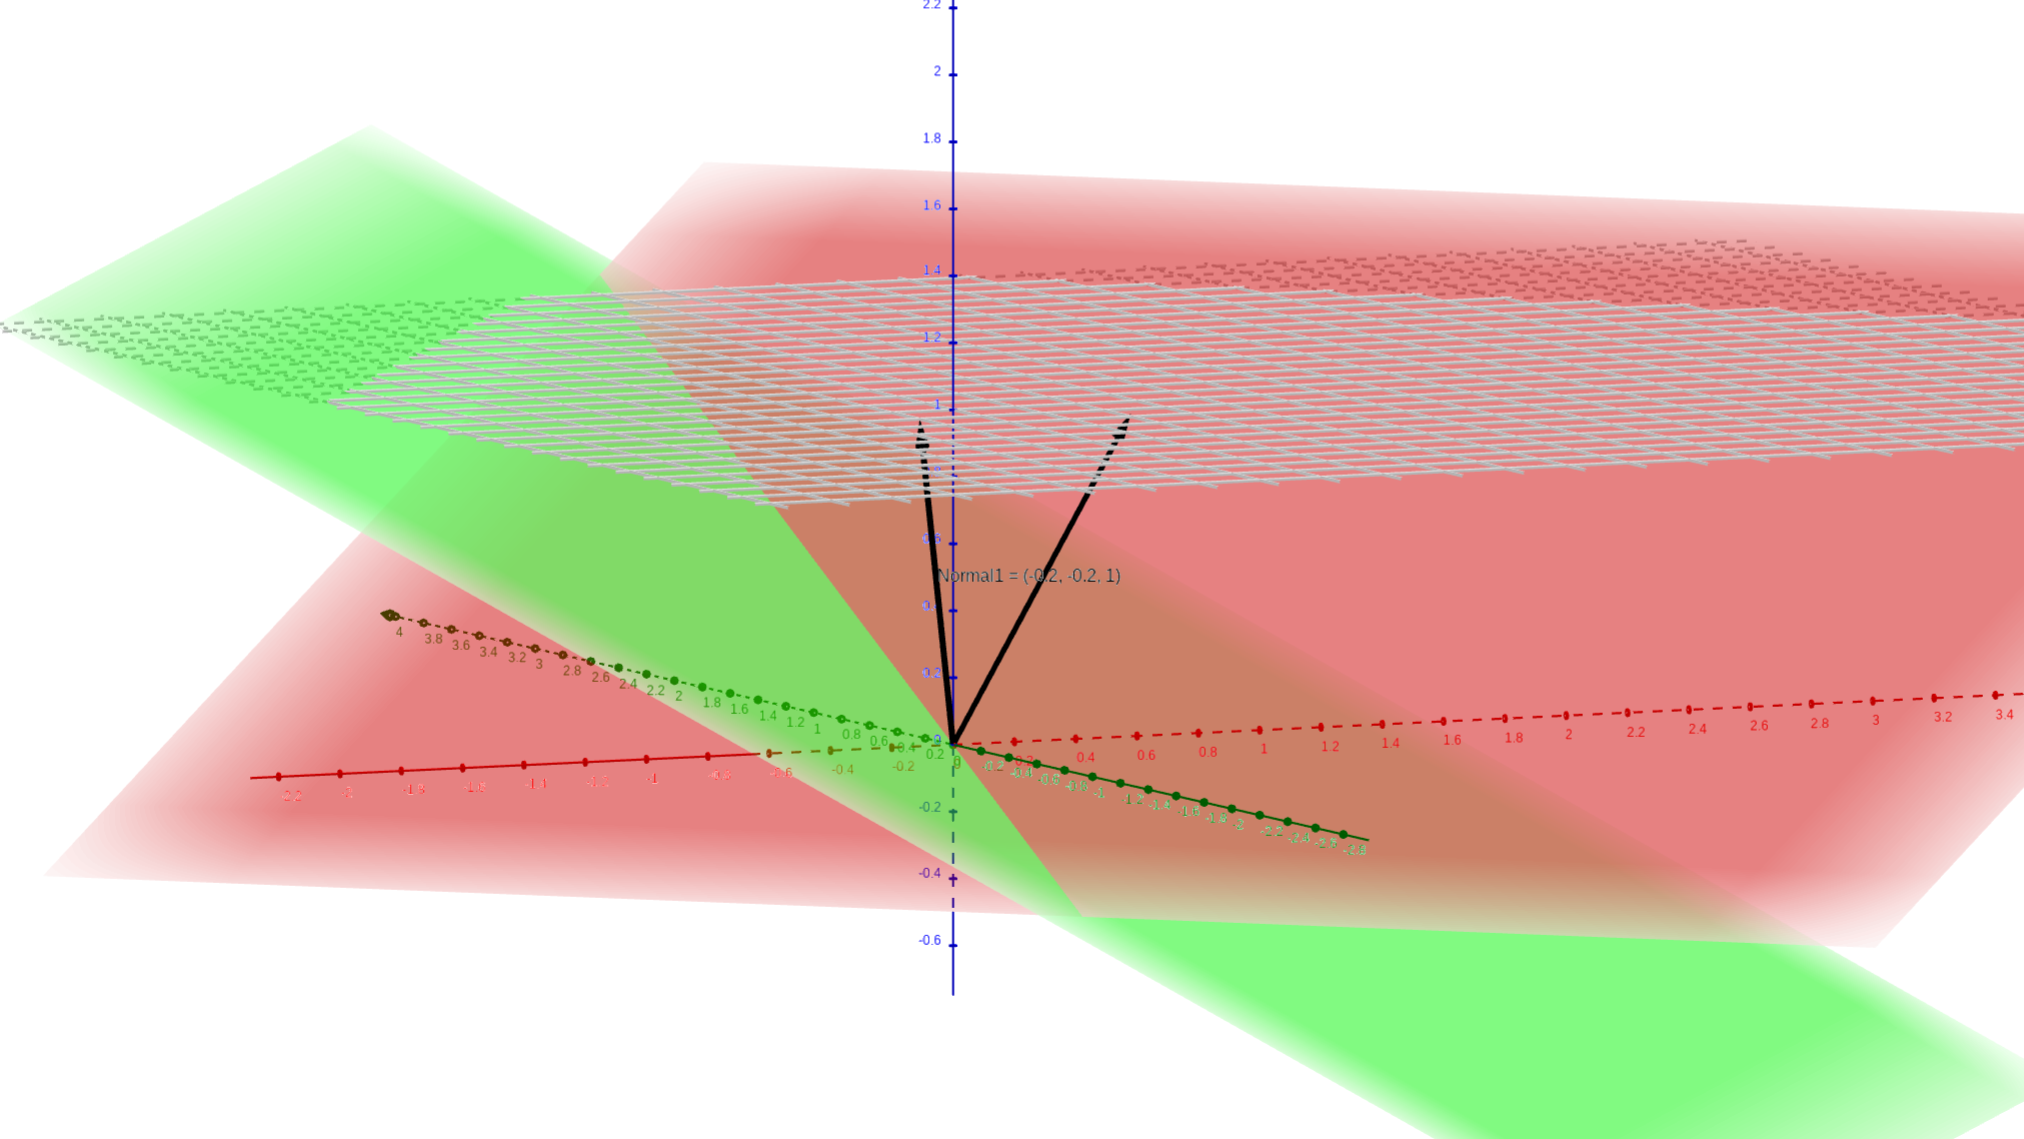
\includegraphics[width=0.49\linewidth]{./res/5.png}
        \caption{Planes definition based on points (left) and their normals
(right)}
        \label{fig:planes}
      \end{figure}

      Once these planes are defined, obtaining a cross product of their normals
should give us a perpendicular vector that is linearly independent and, thus,
contained in both planes! This is seen in \cref{fig:perpendicular}.

      \begin{figure}
        \centering
        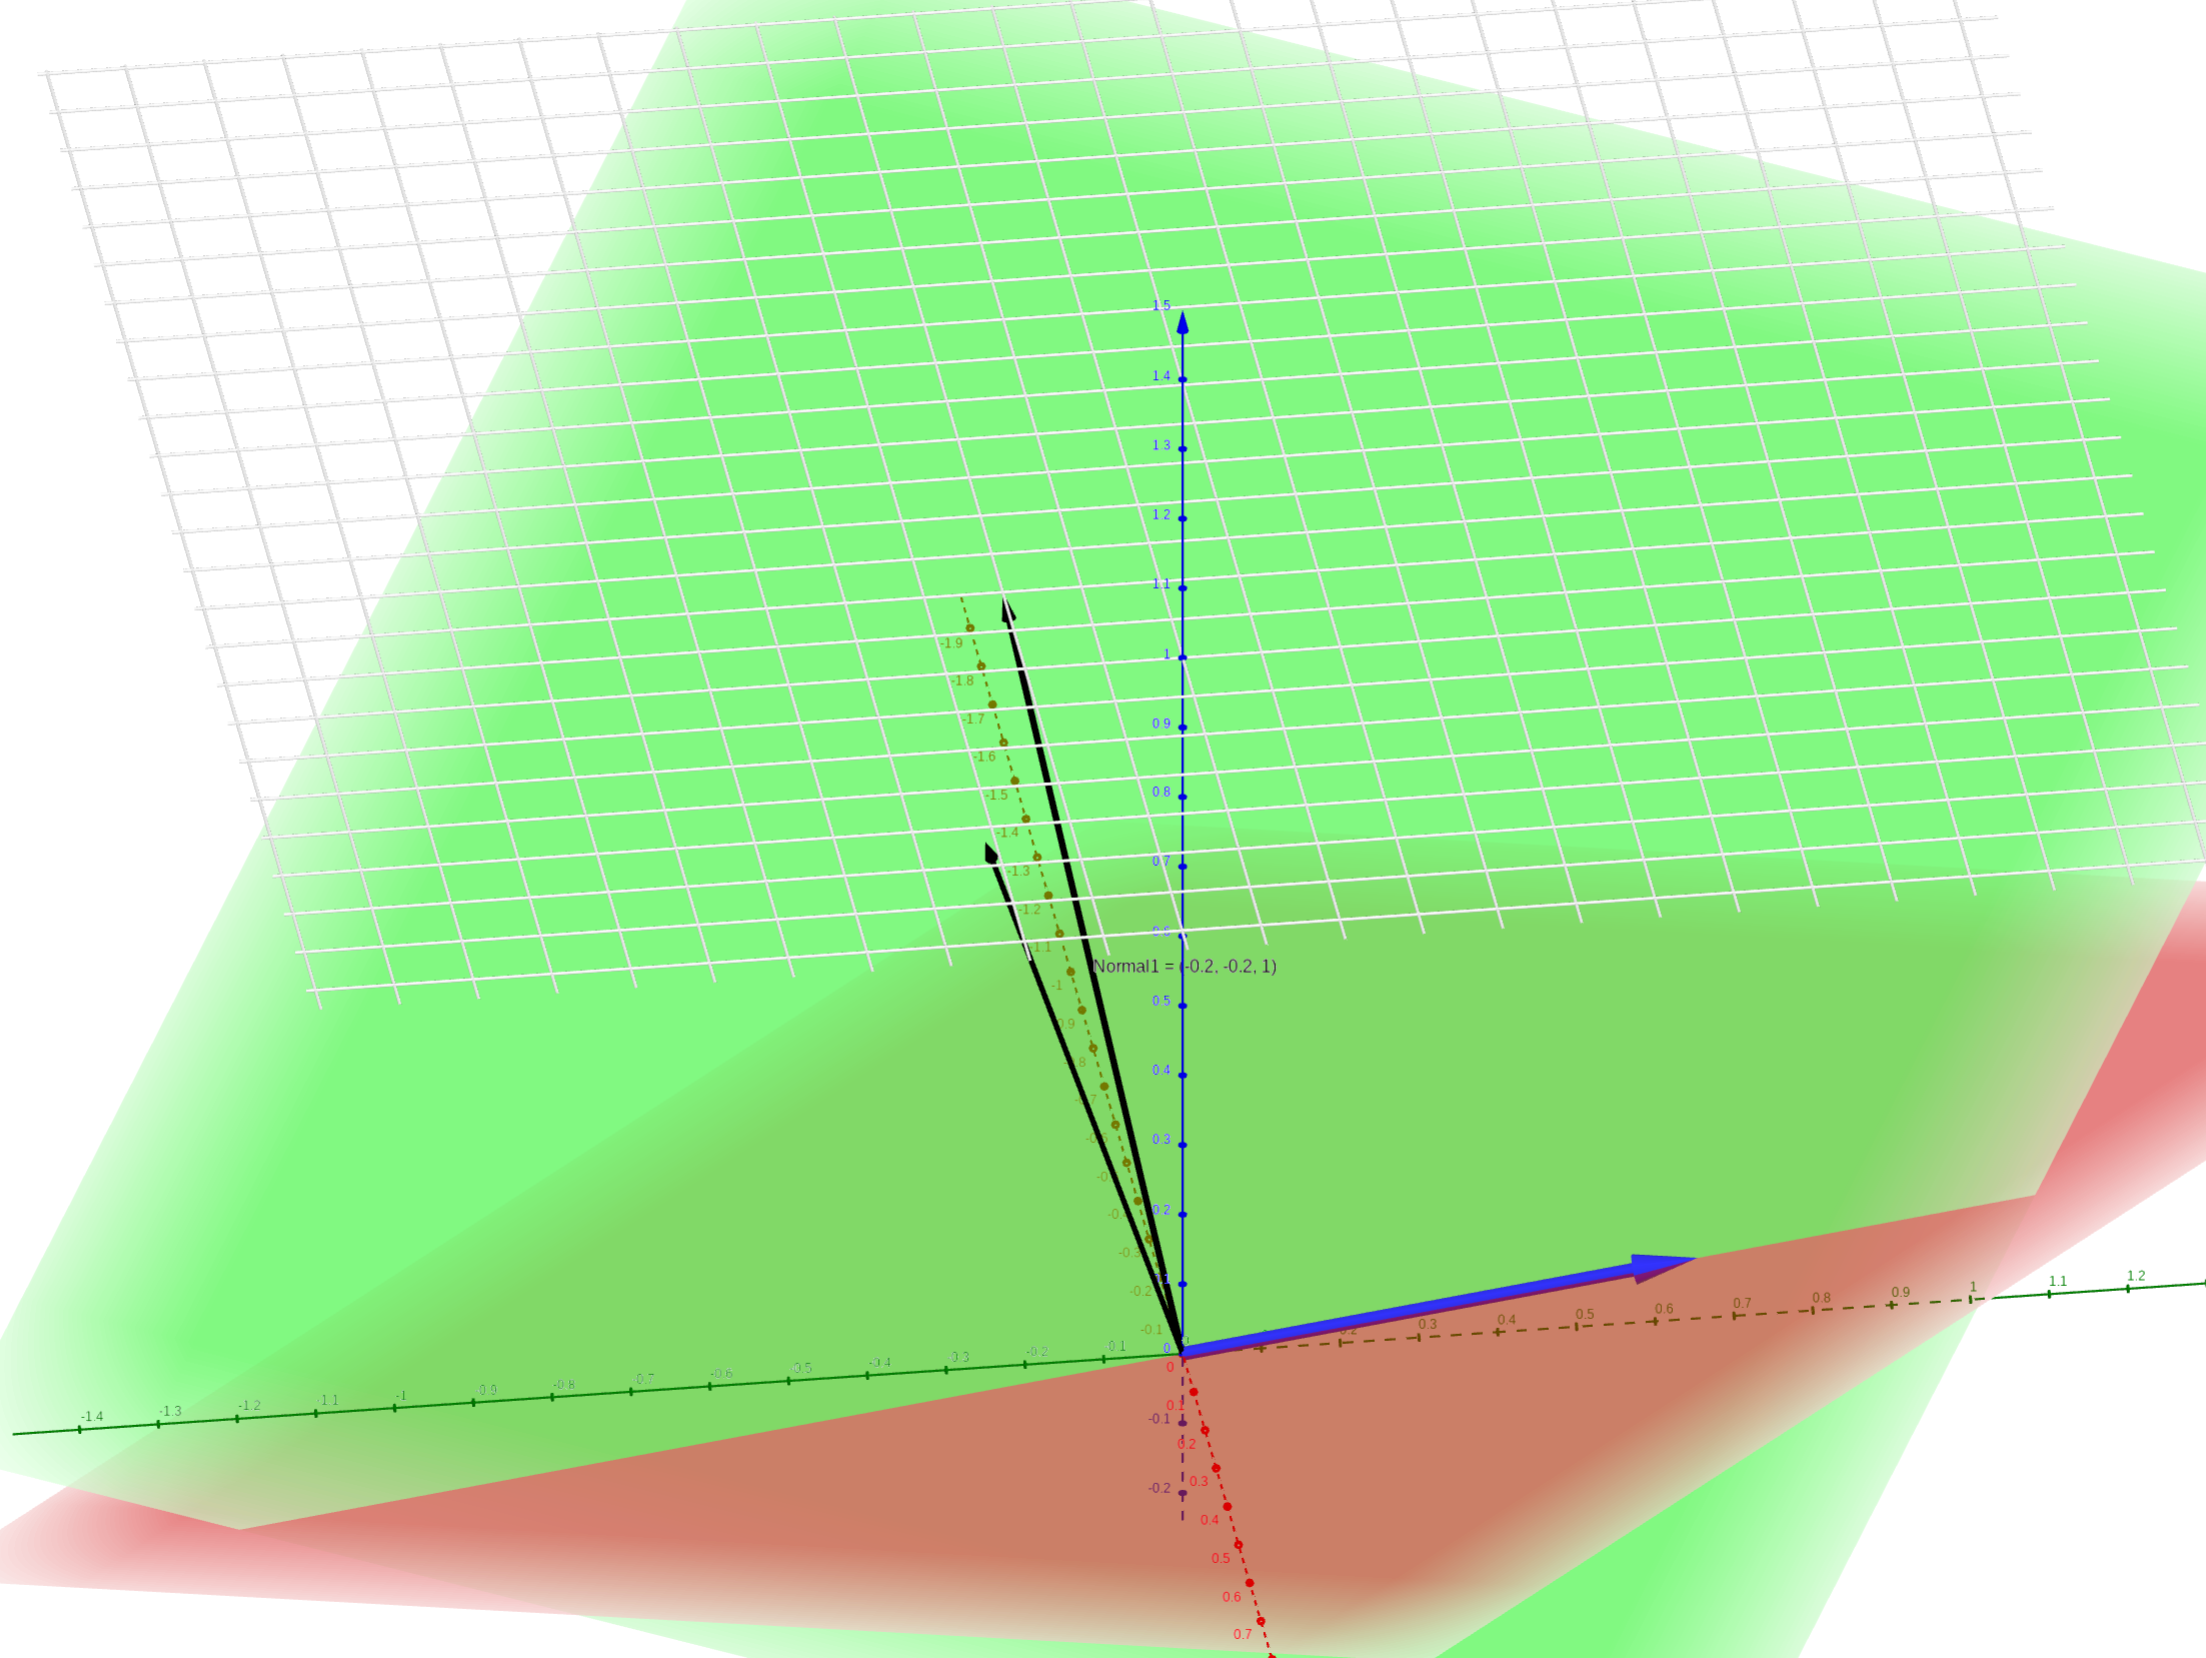
\includegraphics[width=0.49\linewidth]{./res/6.png}
        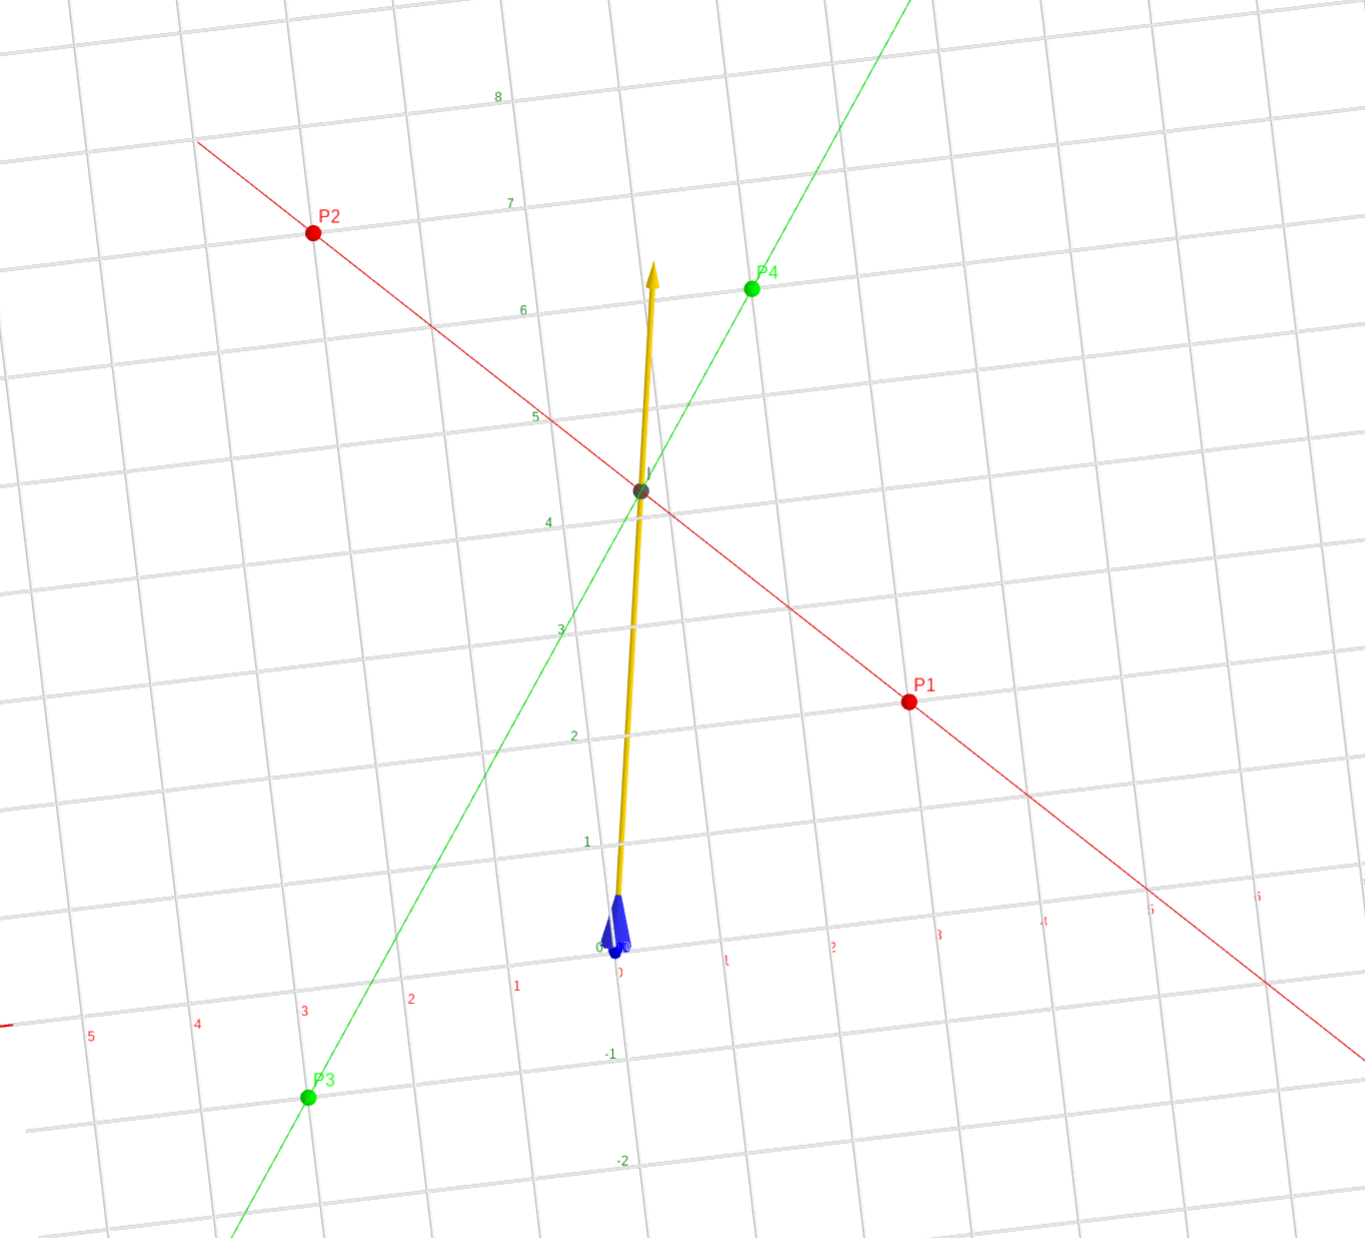
\includegraphics[width=0.49\linewidth]{./res/7.png}
        \caption{Cross product between the two plane normals outlines the
intersection between them (left). Clearly, this outline intersects with the
intersection points defined in \cref{fig:line-intersection} (right).}
        \label{fig:perpendicular}
      \end{figure}

    \end{section}
    \begin{section}{Changing $w$}

      What would happen if we were to change the $w$ value defined in the first
equation set? Reading the homogeneous coordinate $w$ as the value of the points
in the \textit{Z-axis}, we see that by decreasing it, the points would lower
towards the same plane as the origin. This would make it so that the planes
defined in \cref{sec:planes} grow perpendicular. This is shown in
\cref{fig:lower-w}.

      \begin{figure}
        \centering
        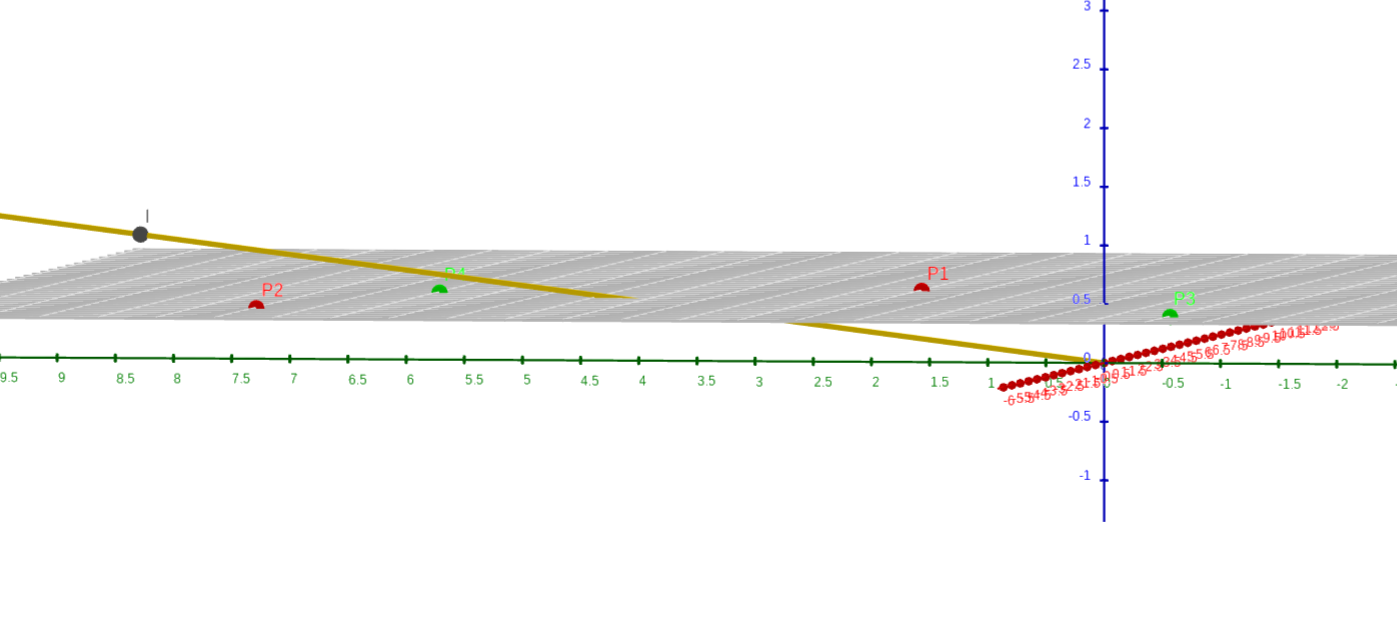
\includegraphics[width=0.85\linewidth]{./res/8.png}
        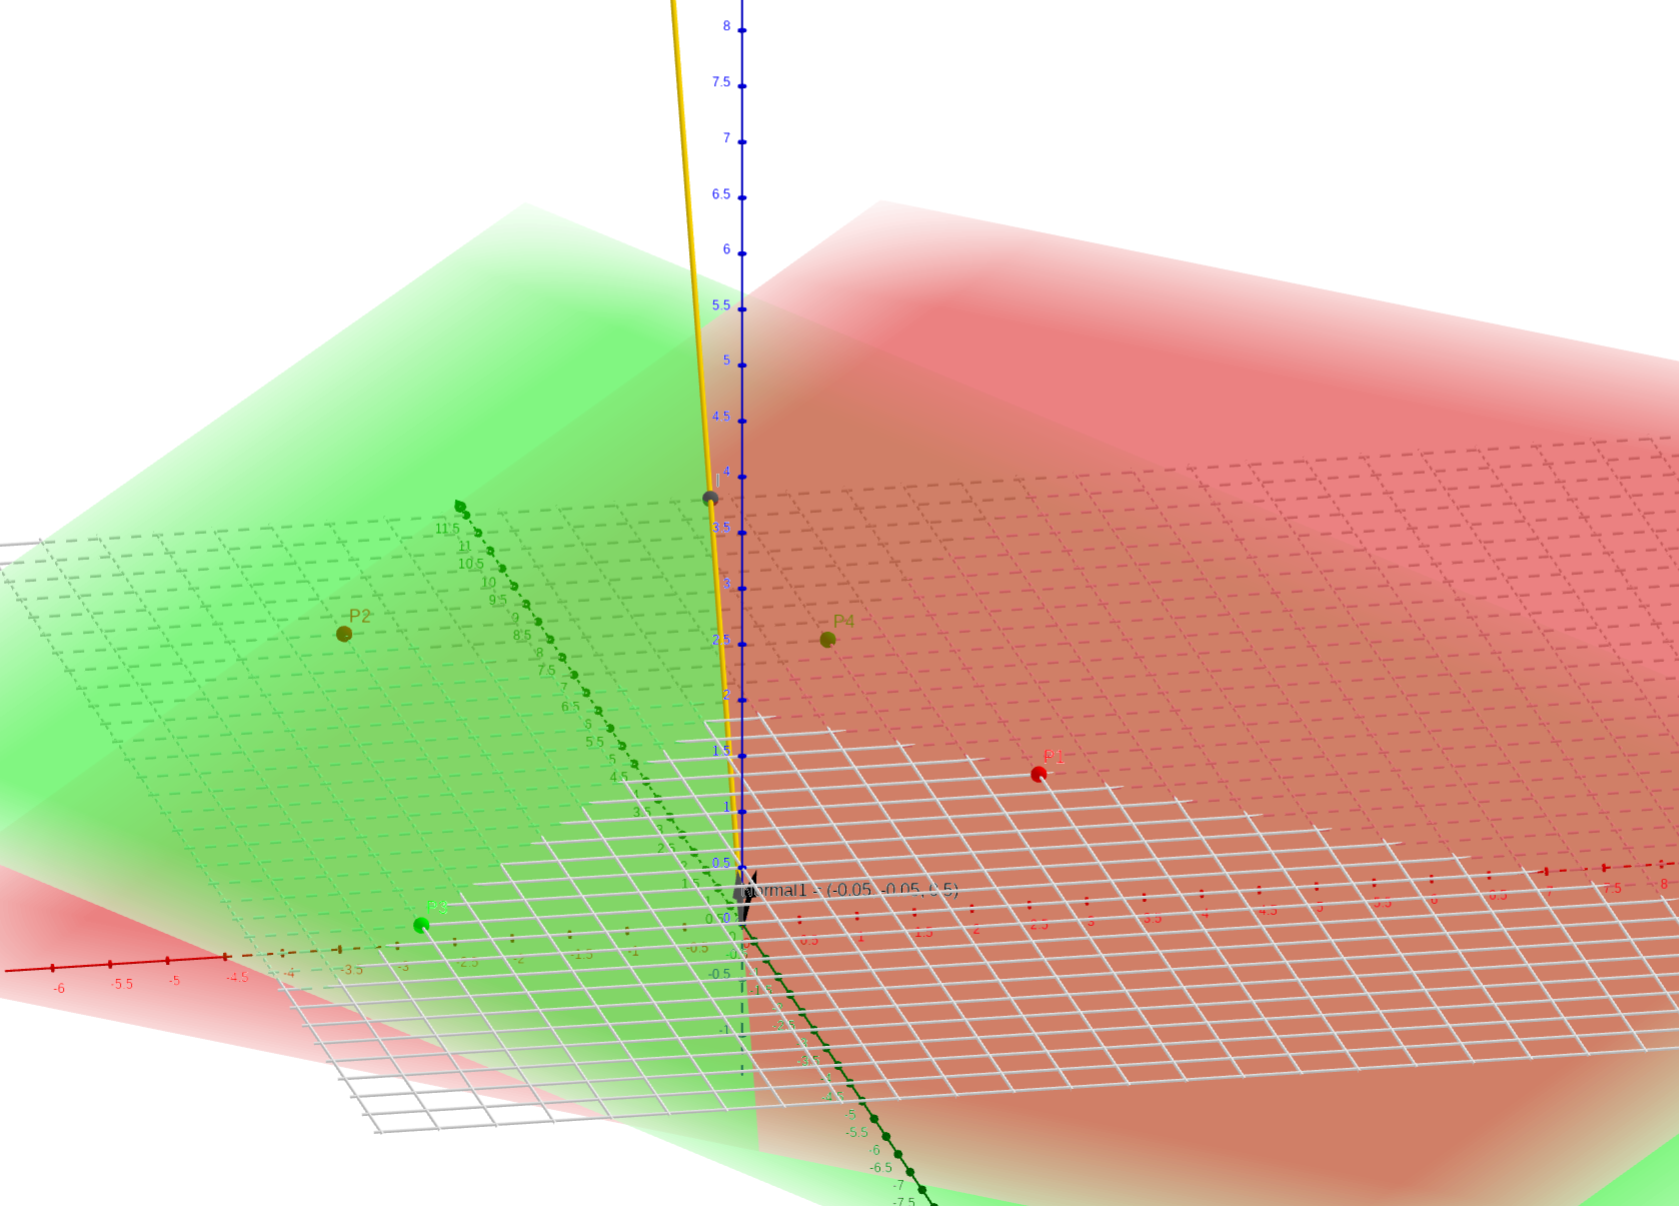
\includegraphics[width=0.85\linewidth]{./res/9.png}
        \caption{As $w$ lowers its value, we see that the calculated
intersection point goes further in the plane outline calculated in
\cref{sec:planes} (top) and that the planes become more alike (bottom).}
        \label{fig:lower-w}
      \end{figure}

    If $w = 0$, it would be natural that the planes become the same and that the
intersection would move towards infinity, as we divide the point by its
homogeneous coordinate to find its position in the $w = 1$ plane.

    \begin{align*}
      [3, 2, 0] \times [-2, 7, 0] &= [0, 0, 25] \\
      [-3, -1, 0] \times [2, 6, 0] &= [0, 0, -16] \\
      [0, 0, 25] \times [0, 0, 16] &= [0, 0, 0] \\
      \text{Intersection Point} &= \frac{[0, 0, 0]}{0}
    \end{align*}
    \end{section}
\end{document}
